\chapter{Online Algorithms}

When dealing with swarms of robots the biggest branch of studies and experiments on this topic usually refers to little robot units with limited sensing, and limited computational capabilities. In this framework simple real time search methods play a significant role since, even if the behaviour of the algorithm itself is not sophisticated, groups of robots take advantage of their collective behaviour, parallelism and fault tolerance. \\
A key concept in swarms behaviour is \emph{stigmergy}, concept at the base of the path planning used in the developed real-time search algorithms.  The stigmergy mechanism allow multiple agents to coordinate indirectly by leaving traces of their movements in the environment. This kind of mechanism is the same used by ants:~they communicate using pheromones trails that are laid and can be followed by other ants. The more ants follow a trace, the more they refresh the pheromone left, and so other ants will follow that path more likely.

We apply the same concept but somehow in a reversed fashion. The terrain is modelled as a grid divided in cells and, since our objective is to perform a complete coverage of the grid, we make our choice by looking at the less visited cells and moving onto them. Both Node Counting and the LRTA* share the same operative work-flow which is synthesised in the following pseudo-code:

\begin{algorithm}
\caption{Navigation Algorithm for the real-time search}
\label{alg:rt_gen}
\begin{algorithmic} [1]
\STATE{$v_c = v_{start}$} \label{a:init_v}
\STATE{$U \leftarrow$ \emph{``set of unvisited vertices''}} \label{a:initU_rt}
\WHILE{$U \neq \emptyset$}\label{a:bigWhile_rt}
	\STATE{$e = choose(v_c, Alg)$} %\COMMENT{$Alg$ determines how the edge is selected.}}
	\STATE{move along edge $e$} %\COMMENT{the robot moves in the Workspace.}}
	\STATE{$v_c := succ(v_c, e)$}
\ENDWHILE
\end{algorithmic}
\end{algorithm}

The three search methods differ only in the \emph{choose} rule which will be discussed in the next sections. 
Let's go through the algorithm: at the beginning a start vertex is assigned (line \ref{a:init_v}) to each quadcopter, and the set $U$ of unvisited vertices is initialised (line \ref{a:initU_rt}). In particular the unvisited set contains all the vertices in the graph with a key value of 0, representing the accessible cells. From this vertex all the neighbour vertices $w_i$ are tested looking at its $c(w_i)$ associated value. We can observe that this methods do not require any memory, since the update rule is just related to the vertex the robot is visiting at a given time and not on the history of its path.

If a robots find itself in a situation where two adjacent vertices happen to have the same value of interest, whether this is a vertex count (Node Counting), an heuristic estimate (LRTA*), and edge count (Edge Counting) or an edge transition probability (PatrolGRAPH*), the robots chooses randomly one of the equally best values. For the multi-robot coverage due to possible communication delays the random factor plays a significant role in spreading out the robots across the map, decreasing the total coverage time.




\section{Node Counting}

Following the logic described in the previous algorithm (\ref{alg:rt_gen}), the Node Counting search updates the vertex count using the following simple rule:

\begin{algorithm}
\begin{algorithmic}[1]
\STATE{$w =$ one-of $arg min_{w_i \in N(v_c)} c(w_i)$} \label{a:find_next_nc}
\STATE{$c(v_c) = 1 + c(v_c)$}\label{eq:nc_rule}
\RETURN{$e(v,w)$}
\end{algorithmic}
\caption{\emph{Choose} operator for Node Counting}\label{alg:rt_nc}
\end{algorithm}


At the beginning of time all the vertices start with a count $c(v)=0$, which means that they are all unvisited vertices. While the robots are exploring the area the Node Counting search make the robots move to the nearest neighbour vertex with the smallest count, so that the swarm agents are automatically steered to the closest unvisited zones. In this way after some time all the vertices will be visited.

\section{Learning Real-Time A*}
\label{sec:LRTAstar}

The update rule of the node Learning Real-Time A* is a little bit less trivial, since is not only based on the current vertex, but also on the successor. The LRTA* algorithm repeats the following steps until the problem solver reaches the goal state. It builds and updates a table containing heuristic estimates of the cost from each state in the problem space. Initially, the entries in the table come from a heuristic evaluation function, or are set to zero if no function is available, and are assumed to be lower bounds of actual costs. Through repeated exploration of the space, however, more accurate values are learned until they eventually converge to the actual costs to the goal \cite{Ishida:1998:RSA:608597.608621}. Its complexity is found to be a small polynomial in n (number of states) \cite{Koenig96easyand}. The vertex count is updated as follows:

\begin{algorithm}
\begin{algorithmic}[1]
\STATE{$w =$ one-of $arg min_{w_i \in N(v_c)} c(w_i)$} \label{a:find_next_lrta}
\STATE{$c_{_{LRTA}}(v) = 1 + c_{_{LRTA}}(w)$}\label{eq:lrta_rule}
\RETURN{$e(v,w)$}
\end{algorithmic}
\caption{\emph{Choose} operator for LRTA*}\label{alg:rt_lrta}
\end{algorithm}

Let's remark first of all that the $c_{_{LRTA}}$ count for this algorithm is not the actual number of visits but an heuristic estimate used for the choosing phase. At the beginning of time all the vertices start with a count $c=0$, which means that they are all unvisited vertices. To understand the mechanism of the LRTA* search, let's imagine to be able to look at a snapshot of the vertices count in the middle of a coverage execution: the $c_{_{LRTA}}(v)$ count value of a vertex $v$ represents the distance from this vertex $v$ to the closest vertex $w$ with $c_{_{LRTA}}(w)$, e.g. an unvisited vertex in a single-coverage case. Since the logic that guides the agent is always to look at the neighbouring vertices with the smallest count, the robot will not only be steered towards the nearest unvisited vertices, but in doing that they will also follow an approximately shortest path.
In \cite{koenig2001} is demonstrated how the LRTA* exhibit better performances than Node Counting for that while in the latter the cover time can be up to exponential in the number of vertices in the graph, the former guaranteed the coverage to be completed in a time polynomial to the number of vertices in the graph.

Despite this the extension of this property from the single-robot case to a multi-robot one is not straightforward and the experimental results for a single-visit coverage show how in some cases Node Counting can be more efficient. This behaviour is related to the update-count rule: while in NC a robot can communicate its vertex choice and consequently update the vertex count in the very same moment he chooses, for the LRTA* a robot has first to reach the vertex and only then it can update its count (since it's related to its next vertex choice). Due do this in LRTA* if many robots are on the same vertex nothing stops them from choosing all the same next vertex, yielding to an inefficient coverage. For single-robot coverage of course this problem does not occur. 


\section{Edge Counting}
The Edge Counting algorithm the count used for making decisions is the edge traversal count of the departing links, from the current position, to the next reachable ones. Supposing we are in vertex $v_c$ where $e_{cj} \in E_c$ form the set of its outgoing edges, the choose operator for this algorithm is:

\begin{algorithm}
\begin{algorithmic}[1]
\STATE{$l =$ one-of $arg min_{j : e_{cj} \in E_c} k_{cj}$} \label{a:find_next_ec}
\STATE{$k_{cl} =k_{cl} + 1$}\label{eq:ec_rule}
\RETURN{$e(c,l)$}
\end{algorithmic}
\caption{\emph{Choose} operator for Edge Counting}\label{alg:rt_ec}
\end{algorithm}

$k_{ij}$ is the edge count, an integer variable initialized to $0$ which counts the number of times that robots have chosen to proceed to $v_j$ after leaving $v_i$. In general, no real-time search algorithm can beat the complexity of LRTA*, which is a small polynomial in n. In contrast, the deterministic Edge Counting that we derived from random walks has a complexity that is at least exponential in n. The picture changes in Eulerian state spaces. The complexity of edge counting decreases dramatically and equals the complexity of LRTA*, which remains unchanged (it even beats LRTA* in certain specific domains) \cite{Koenig96easyand}. 


\section{PatrolGRAPH*}

The logic behind the PatrolGRAPH* follows a different approach. First of all, although it is presented as online algorithm, it also presents an offline phase which is needed in order to optimise the successive online phase. So we can classify it in the middle of the two approaches. It takes into account not only information about the vertex count, but also on the edge traversal count. In particular the decision that is made in vertex $v_i$ to choose the next vertex $v_j$ is based on the probability associated to the edge that connects them $e(i,j)$.
The algorithm is designed to solve the problem of Multi--Robot Controlled Frequency Coverage, in which a team of robots are requested to repeatedly visit a set of pre--defined locations of the environment according to a specified \emph{frequency distribution}. In particular we want the frequency distribution to be \emph{uniform} in order to visit all the vertices of the graph in the shortest time, and this kind of formulation is known as the Multi--Robot Uniform Frequency Coverage (MRUFC). In particular the MRUFC problem corresponds to the case when ${\bm{\lambda}}^*$ has a uniform distribution, i.e., for all $s_i$, $\lambda_i^* = 1/N$.  The frequency distribution of visits in particular is controlled by tuning the so called \emph{transition matrix} $P$, which contains for each edge $e_{ij}$ the probability $p_{ij}$ of being traversed. $P$ is subject to the following constraints:

\begin{equation}
\sum\limits_{j=1}^{N} {p_{ij} } = 1, \quad (i=1,\ldots,N),
\label{Pmatrix3b}
\end{equation}

\begin{equation}
0 \leq p_{ij} \leq 1,\quad (i,j=1,\ldots,N). 
\label{Pmatrix3c}
\end{equation}
 
In its simplest form the elements of $P$ will be:

\begin{equation}
p_{ij}=\frac{1}{|E_i|},
\label{eq_adj}
\end{equation}
if $v_i$ and $v_j$ are adjacent, while if $s_i$ and $s_j$ are not adjacent,
\begin{equation}
p_{ij}=0.
\label{eq_noadj}
\end{equation}

It is easy to understand that with this kind of formulation every vertex will receive a number of visits which is proportional to its incoming edges, and we want instead all the vertices to be visited uniformly. To accomplish this the PatrolGRAPH* performs the so called \emph{offline phase} to tune the $P$ transition matrix.

%%%%%%%%%%%%%%%%%%%%%%%%%%%%%%
\subsection{The offline phase}

Let $\bm{1}=[1 \ldots 1]^T$ be the unitary vector. The flow balance equations in matrix form, by considering the additional requirement that the sum of average visiting rates, computed over all vertices of $\hat{G}_N$, is constant, can be written as:

\begin{equation}
\left[\begin{array}{*{20}c} {P^T - I} \\ {\bm 1^T} \end{array} \right] \bm \lambda = \left[\begin{array}{*{20}c} {0} \\ \vdots \\ {0} \\ {C} \end{array}\right].
\label{theorem45}
\end{equation}

The system \eqref{theorem45} has exactly one solution whenever $P$ is stochastic and irreducible \cite{5711675}. The last equation in \eqref{theorem45} allows one to determine the unique solution whose components sum up to $C$.

The off--line phase then has the main purpose of finding a solution to the so--called \emph{inverse problem}, i.e., the problem of choosing $P$ such as to guarantee that the solution of \eqref{theorem45}, with $C=1$, corresponds to the prescribed frequency distribution. The off--line phase does not involve the individual robots.

Let ${\bf{b}} = [b_{1}\cdots b_{N^2}]^T\in \Re^{N^2}$ be defined as a vector which parametrize the elements of the transition matrix $P$, so that $P=P({\bf{b}})\in\Re^{N\times N}$. This is done by ideally subdividing $\bf{b}$ into $N$ vectors with length $N$, and by stacking them onto each other to build up the rows of $P$. More formally, 
\begin{equation}
p_{ij}=b_{N \times (i - 1) + j}, \quad (i,j=1,\ldots,N),
\label{ths0}
\end{equation}

and $\bm{\lambda^*}$ represent the ideal desired solution of the MRCFC problem. Then, ${\bm{\lambda^*} - \bm{\lambda}({\bf{b}})}$ is a representation of the mismatch between the actual frequency distribution and the desired one as a function of the structure of the navigation graph (expressed by the entries of matrix $P$). 

The off--line phase of the \textit{PatrolGRAPH*} algorithm is the search for a solution to the following minimization problem with respect to the unknown variable ${\bf{b}}$.


\begin{equation}
{\bf{b^*}} = \arg \min_{{\bf{b}}}({\bm{\lambda^*} - \bm{\lambda}({\bf{b}})})^T ({\bm{\lambda^*} - \bm{\lambda}({\bf{b}})}),
\label{ths3}
\end{equation}
\indent subject to
\begin{equation}
\sum\limits_{j=1}^{N} {b_{N\times(i-1)+j} } = 1, \quad (i=1,\ldots,N), \\
\label{con3a}
\end{equation}
\begin{equation}
b_{N\times(i-1)+j} \ge  |\epsilon |,\quad (\forall i,j\quad s.t.\quad a_{ij} \in A_i),  
\label{con3b}
\end{equation}
\begin{equation}
b_{N\times(i-1)+j} = 0,\quad (\forall i,j\quad s.t.\quad a_{ij} \notin A_i). 
\label{con3c}
\end{equation}


%%%%%%%%%%%%%%%%%%%%%%%%%%%%%%
\subsection{The online phase}
After performing the previous steps, the online phase follows the same pattern of the previous ones as in Algorithm \ref{alg:rt_gen}, but now the choose operator is more elaborated:

\begin{algorithm}
\begin{algorithmic}[1]
\STATE{$c(v) = c(v) + 1$} \label{a:PG_upd_cv}
\FORALL{$j$ such that $e_{cj}\in E_c$} %\label{a:initU_rt}
	\STATE{$\Delta p_{cj} = (k_{cj}- \eta_{j})/v_c - p_{cj}$}\label{a:PG_deltaP}
\ENDFOR
\STATE{$l = arg min_{j}( \Delta p_{cj})$}\label{a:PG_find_min}
\STATE{$k_{cl} = k_{cl} + 1$}\label{a:PG_upd_k}
\RETURN{$e_{cl}$}
\end{algorithmic}
\caption{Choose operator for PatrolGRAPH*}\label{alg:rt_pg}
\end{algorithm}

Where: $c(v)$ same as before is the vertex count. $k_{ij}$ is the edge count. $\eta_j$ is a zero mean random variable with standard deviation $\sigma$, that is, $\eta_j=N(0,\sigma)$. In particular $\eta$ is used to purposely introduce a factor of unpredictability but since we don't need this feature we will simply set it to zero. Line \ref{a:PG_upd_cv} updates the number of visits $c(v)$ received by $v_c$; Line \ref{a:PG_deltaP} computes, for every adjacent vertex, the error $\Delta p_{cj}$ between the ratio $k_{cj}/v_c$ and the desired relative frequency $p_{cj}$; Line \ref{a:PG_find_min} picks the edge $a_{cl}$ for which $\Delta p_{cj}$ is minimum; Line \ref{a:PG_upd_k} updates $k_{cl}$. 
In \cite{5711675} is demonstrated that the routing policy adopted by \textit{PatrolGRAPH*} in Algorithm \ref{alg:rt_pg} to distribute robots along edges $a_{ij}$ departing from $s_i$ converges to the desired relative frequencies $p_{ij}$.

To demonstrate the effectiveness of the offline phase of the PatrolGRAPH* the algorithm is tested on a 5x5 grid obstacle-free map (cell side size 5 m) using 3 quadcopters, running four simulations with two different time horizons: 

\begin{itemize}
\item 10 minutes patrolling without and with (figures \ref{fig:PG_pic1} and \ref{fig:PG_pic2})
\item 20 minutes patrolling without and with (figures \ref{fig:PG_pic3} and \ref{fig:PG_pic4})
\end{itemize}

The figures mentioned in the list are a graphical representation of the visit count for the cells in the map. In particular the visit count is encoded as a colour and the colour-bar is the reference. First of all it is important to know that the starting point for all the quadcopters is the cell in position (2,0), and this of course affects the propagation of visit in the neighbouring cells. In Figure \ref{fig:PG_pic1} and \ref{fig:PG_pic3} we can observe how without running the offline phase the corner vertices, which have the lowest number of in-going edges, receive a significantly smaller amount of visits (colour near blue).  In Figure \ref{fig:PG_pic2} and \ref{fig:PG_pic4}, instead, we notice how the visit distribution is much more uniform, and as the simulation time increases the coverage becomes more uniform.
\begin{figure}[h] 
  \label{fig:PG_countMaps}
  \centering
  \begin{minipage}[b]{0.45\linewidth}
    \centering
    % This file was created by matlab2tikz v0.4.7 running on MATLAB 8.0.
% Copyright (c) 2008--2014, Nico Schlömer <nico.schloemer@gmail.com>
% All rights reserved.
% Minimal pgfplots version: 1.3
% 
% The latest updates can be retrieved from
%   http://www.mathworks.com/matlabcentral/fileexchange/22022-matlab2tikz
% where you can also make suggestions and rate matlab2tikz.
% 

\begin{tikzpicture}
\begin{axis}[%
width=.75\linewidth,
%height=3.565625in,
axis on top,
%scale only axis,
xtick={0,1,...,4},
ytick={0,1,...,4},
xmin=-0.5,
xmax=4.5,
y dir=reverse,
ymin=-0.5,
ymax=4.5,
colormap/jet,
colorbar,
point meta min=0,
point meta max=19
]
\addplot [forget plot] graphics [xmin=-0.5,xmax=4.5,ymin=-0.5,ymax=4.5] {img/tikzPlots/5x5_unoptim_10min.png};
\end{axis}
\end{tikzpicture}%
    \caption{Unoptimised PG* 10 min}
    \label{fig:PG_pic1}
    \vspace{4ex}
  \end{minipage}
  \quad
  \begin{minipage}[b]{0.45\linewidth}
    \centering
    % This file was created by matlab2tikz v0.4.7 running on MATLAB 8.0.
% Copyright (c) 2008--2014, Nico Schlömer <nico.schloemer@gmail.com>
% All rights reserved.
% Minimal pgfplots version: 1.3
% 
% The latest updates can be retrieved from
%   http://www.mathworks.com/matlabcentral/fileexchange/22022-matlab2tikz
% where you can also make suggestions and rate matlab2tikz.
% 
\begin{tikzpicture}

\begin{axis}[%
width=.75\linewidth,
%height=3.565625in,
axis on top,
%scale only axis,
xtick={0,1,...,4},
ytick={0,1,...,4},
xmin=-0.5,
xmax=4.5,
y dir=reverse,
ymin=-0.5,
ymax=4.5,
colormap/jet,
colorbar,
point meta min=0,
point meta max=18
]
\addplot [forget plot] graphics [xmin=-0.5,xmax=4.5,ymin=-0.5,ymax=4.5] {img/tikzPlots/5x5_optim_10min.png};
\end{axis}
\end{tikzpicture}%
    \caption{Optimised  PG* 10 min}
    \label{fig:PG_pic2}
    \vspace{4ex}%%
  \end{minipage}
  \begin{minipage}[b]{0.45\linewidth}
    \centering
    % This file was created by matlab2tikz v0.4.7 running on MATLAB 8.0.
% Copyright (c) 2008--2014, Nico Schlömer <nico.schloemer@gmail.com>
% All rights reserved.
% Minimal pgfplots version: 1.3
% 
% The latest updates can be retrieved from
%   http://www.mathworks.com/matlabcentral/fileexchange/22022-matlab2tikz
% where you can also make suggestions and rate matlab2tikz.
% 
\begin{tikzpicture}

\begin{axis}[%
width=.75\linewidth,
%height=3.565625in,
axis on top,
%scale only axis,
xtick={0,1,...,4},
ytick={0,1,...,4},
xmin=-0.5,
xmax=4.5,
y dir=reverse,
ymin=-0.5,
ymax=4.5,
colormap/jet,
colorbar,
point meta min=0,
point meta max=32
]
\addplot [forget plot] graphics [xmin=-0.5,xmax=4.5,ymin=-0.5,ymax=4.5] {img/tikzPlots/5x5_unoptim_20min.png};
\end{axis}
\end{tikzpicture}%
    \caption{Unoptimised  PG* 20 min} 
    \label{fig:PG_pic3}
    \vspace{4ex}
  \end{minipage}
  \quad
  \begin{minipage}[b]{0.45\linewidth}
    \centering
    % This file was created by matlab2tikz v0.4.7 running on MATLAB 8.0.
% Copyright (c) 2008--2014, Nico Schlömer <nico.schloemer@gmail.com>
% All rights reserved.
% Minimal pgfplots version: 1.3
% 
% The latest updates can be retrieved from
%   http://www.mathworks.com/matlabcentral/fileexchange/22022-matlab2tikz
% where you can also make suggestions and rate matlab2tikz.
% 
\begin{tikzpicture}

\begin{axis}[%
width=.75\linewidth,
%height=3.565625in,
axis on top,
%scale only axis,
xtick={0,1,...,4},
ytick={0,1,...,4},
xmin=-0.5,
xmax=4.5,
y dir=reverse,
ymin=-0.5,
ymax=4.5,
colormap/jet,
colorbar,
point meta min=0,
point meta max=26
]
\addplot [forget plot] graphics [xmin=-0.5,xmax=4.5,ymin=-0.5,ymax=4.5] {img/tikzPlots/5x5_optim_20min.png};
\end{axis}
\end{tikzpicture}%
    \caption{Optimised  PG* 20 min}
    \label{fig:PG_pic4}
    \vspace{4ex}%% 
  \end{minipage} 
\end{figure}

\pagebreak

\section{Implementation}

For the online algorithms the map count values (visit count and edge traversal) are updated by means of the ROS network. Taking the LRTA* algorithm as an example, each node is at a same time publishing and subscribed to the same common topic  \textit{updateLRTACount}, and each time one of the agents publishes on it, all of them updates the counts in their grid.
All the control \emph{quadLRTAstar} nodes are launched together using the \texttt{roslaunch} package. Each time a robot is about to move it check whether all the nodes have been visited, and if the unvisited set is empty the robots stop searching.
As you can see in Fig. \ref{fig:rt_nodes} all the ROS nodes are independent, but they communicate through the common topic. This node network is relative to the LRTA* algorithm, but the same scheme holds also for all the other online algorithms.

\begin{figure}[h]
\centering
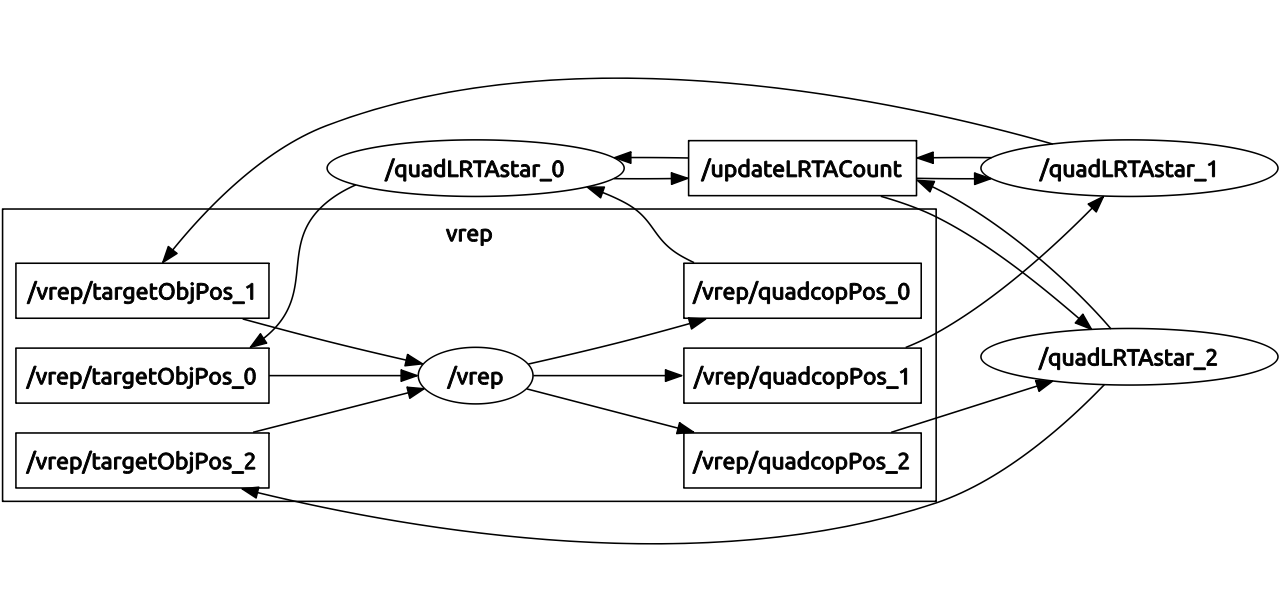
\includegraphics[scale=0.3]{swarm_LRTAstar}
\caption[ROS network for the online algorithms]{The nodes and topics ROS network of the online algorithms. The ellipses are nodes while the rectangles are topics.}
\label{fig:rt_nodes}
\end{figure}




